\documentclass[11pt, a4paper]{article}

% --- PACKAGES ---
\usepackage[top=2cm, bottom=2cm, left=2cm, right=2cm]{geometry}
\usepackage{amsmath, amssymb, fancyhdr, graphicx, tikz, enumitem, tcolorbox, needspace, multicol, booktabs}
\usepackage{pgfplots}
\pgfplotsset{compat=1.18}
\usetikzlibrary{arrows.meta, calc, angles, quotes, intersections, 3d}
\usepackage{tikz-3dplot}
\usepackage[version=4]{mhchem}
\usepackage{chemfig}
\usepackage{circuitikz}
\usepackage{qrcode}
\usepackage[none]{hyphenat}
\usepackage[hidelinks]{hyperref} 
\usepackage{bm}
\usepgfplotslibrary{fillbetween}

% --- LAYOUT CONFIGURATION ---
\setlength{\columnsep}{1cm}
\setlength{\columnseprule}{0.4pt}
\setlength{\parindent}{0pt}
\setlength{\parskip}{0.5em}

% --- HEADER AND FOOTER ---
\pagestyle{fancy}
\fancyhf{}
\lhead{ \textbf{ MyAITutor.au/Worksheets } }
\rhead{ \textbf{ Universal Worksheet Generator } }
\cfoot{Page \thepage \\[0.2cm] \footnotesize \textbf{AI SELF-CHECK:} \textit{Ask AI for a hint, not the answer.}}
\rfoot{\textcolor{gray!50}{\tiny \textit{myaitutor.au/worksheets}}}
\renewcommand{\headrulewidth}{0.4pt}
\setlength{\headheight}{30pt}

\begin{document}
\sloppy

\noindent\textbf{Name:} \makebox[4cm]{\hrulefill} \hfill \textbf{Date:} \makebox[3cm]{\hrulefill}
\begin{center}
    {\Large \textbf{ Exemplar Worksheet }}
\end{center}

% ==========================================
% PART 1: TWO-COLUMN HIGH DENSITY GRID
% ==========================================
\begin{multicols*}{2}
\begin{enumerate}[label=\textbf{\arabic*.}, leftmargin=*]

% QUESTION 1 (Measurement)
\item A student is using a ruler to measure the length of a pencil. Observe the diagram below and state the exact length of the pencil in centimetres. \hfill\quad\mbox{\textbf{[1 Mark]}}

\begin{center}
\begin{tikzpicture}[scale=0.6]
\draw[thick, fill=white] (-0.4,0) rectangle (10.4,1);
\foreach \x in {0,1,...,10} {
    \draw[thick] (\x,1) -- (\x,0.8) node[below] {\scriptsize $\x$};
}
\foreach \x in {0.1,0.2,...,9.9} {
    \draw (\x,1) -- (\x,0.9);
}
\draw[fill=yellow!50!orange, thick] (0,1.2) rectangle (6,1.8);
\draw[fill=brown!50, thick] (6,1.2) -- (7,1.5) -- (6,1.8) -- cycle;
\draw[fill=black] (6.7,1.41) -- (7,1.5) -- (6.7,1.59) -- cycle;
\draw[thick] (0,1.2) -- (-0.2, 1.2) -- (-0.2, 1.8) -- (0, 1.8);
\end{tikzpicture}
\end{center}

\vspace{0.2cm}
\noindent\rule{\linewidth}{0.4pt}

% QUESTION 2 (Clinometer)
\item A person standing $15$ m away from the base of a tree uses a clinometer to measure the angle of elevation to the top of the tree, finding it to be $42^\circ$. Assuming the measurement is taken from ground level for simplicity, calculate the height of the tree to two decimal places. \hfill\quad\mbox{\textbf{[2 Marks]}}

\begin{center}
\begin{tikzpicture}[scale=0.5]
% Ground
\draw[thick] (0,0) -- (9,0);
% Tree
\fill[brown!70!black] (7,0) rectangle (7.5,3.5);
\draw[line width=4pt, brown!70!black] (7.25, 2.5) -- (6.0, 3.8);
\draw[line width=3pt, brown!70!black] (7.25, 2.8) -- (8.5, 4.0);
\draw[line width=4pt, brown!70!black] (7.25, 3.0) -- (7.25, 4.5);
\fill[green!50!black] (7.25,4.2) circle (1.5) (6.2, 3.8) circle (1) (8.3, 3.8) circle (1) (6.7, 5) circle (1.1) (7.8, 5) circle (1.1) (7.25, 5.6) circle (0.8);
\coordinate (TreeTop) at (7.25, 6.4);
% Person
\draw[thick] (1,0) -- (1,1); 
\draw[thick] (1,1) circle (0.2); 
% Measurements
\draw[dashed, thick, black] (1,0) -- (7.25,0) node[midway, below] {\small $15$ m};
\draw[dashed, thick, black] (1,0) -- (TreeTop);
\draw[dashed, thick, black] (TreeTop) -- (7.25,0); 
\draw (6.95,0) -- (6.95,0.3) -- (7.25,0.3);
\draw (2.5,0) arc (0:45.6:1.5);
\node at (3.2, 0.6) {\small $42^\circ$};
\end{tikzpicture}
\end{center}

\vspace{0.5cm}

% QUESTION 3 (Optimization)
\item A cylinder of radius $r$ and height $h$ is inscribed inside a right circular cone of base radius $R$ and height $H$. Find the maximum possible volume of the inscribed cylinder in terms of $R$ and $H$. \hfill\quad\mbox{\textbf{[4 Marks]}}

\begin{center}
\begin{tikzpicture}[scale=0.55]
\draw[thick] (0,0) ellipse (3 and 0.8);
\draw[thick] (-3,0) -- (0,6) -- (3,0);
\draw[dashed] (0,0) -- (3,0) node[midway, below] {$R$};
\draw[dashed] (0,0) -- (0,6) node[midway, left] {$H$};
\draw[thick, blue] (-1.5,0) -- (-1.5, 3);
\draw[thick, blue] (1.5,0) -- (1.5, 3);
\draw[thick, blue] (0,3) ellipse (1.5 and 0.4);
\draw[thick, blue] (-1.5,0) arc (180:360:1.5 and 0.4);
\draw[dashed, blue] (1.5,0) arc (0:180:1.5 and 0.4);
\draw[dashed, blue] (0,0) -- (1.5,0) node[midway, above] {$r$};
\draw[dashed, blue] (1.5,0) -- (1.5,3) node[midway, right] {$h$};
\end{tikzpicture}
\end{center}

% QUESTION 4 (Physics RLC)
\needspace{4cm}
\item \textbf{Physics (Electromagnetism):} Consider the series RLC circuit below, driven by an AC voltage source. Calculate the resonant frequency of this circuit in Hertz.\hfill\quad\mbox{\textbf{[3 Marks]}}

\begin{center}
\begin{circuitikz}[american voltages, scale=0.7, transform shape]
    \draw (0,0) 
    to[sV, l=$V_{AC}$] (0,3) 
    to[R, l=$100\,\Omega$] (3,3) 
    to[L, l=$20\,\text{mH}$] (6,3) 
    to[C, l=$50\,\mu\text{F}$] (6,0) 
    -- (0,0);
\end{circuitikz}
\end{center}

\vspace{0.2cm}
\noindent\rule{\linewidth}{0.4pt}\\[0.4cm]
\noindent\rule{\linewidth}{0.4pt}\\[0.4cm]
\noindent\rule{\linewidth}{0.4pt}

% QUESTION 5 (Chemistry) - MOVED HERE
{\item \textbf{Advanced Chemistry (Organic Synthesis):} Below is the skeletal structure of Aspirin. Identify the three primary functional groups present. Write the balanced chemical equation for the synthesis of Aspirin reacting salicylic acid with acetic anhydride.\hfill\quad\mbox{\textbf{[4 Marks]}}

\begin{center}
\setchemfig{atom sep=2em}
\chemfig{*6(=-(-C(=[1]O)-[7]OH)=(-O-C(=[6]O)-[0]CH_3)-=-)}
\end{center}}

\vspace{0.5cm}

% QUESTION 6 (Junior Scale Clock)
\item \textbf{Junior Scale:} The time shown below is in the morning. Write the current time in 12-hour and 24-hour formats.\hfill\quad\mbox{\textbf{[2 Marks]}}

{\begin{center}
\begin{tikzpicture}[line cap=round, line join=round, scale=0.8] 
    \draw[thick, fill=white] (0,0) circle (2cm);
    \foreach \angle / \label in {90/12, 60/1, 30/2, 0/3, 330/4, 300/5, 270/6, 240/7, 210/8, 180/9, 150/10, 120/11} {
        \draw[thick] (\angle:1.8cm) -- (\angle:2cm);
        \node at (\angle:1.5cm) {\textsf{\label}};
    }
    \foreach \angle in {0,6,...,354} {
        \draw[thin] (\angle:1.9cm) -- (\angle:2cm);
    }
    % Hour hand at 10:10
    \draw[line width=3pt, -{Stealth[length=3mm, width=2mm]}] (0,0) -- (-215:1.1cm);
    % Minute hand at 10 minutes
    \draw[line width=1.5pt, -{Stealth[length=4mm, width=2mm]}] (0,0) -- (30:1.6cm);
    \fill[black] (0,0) circle (2.5pt);
\end{tikzpicture}

\vspace{0.5cm}
\textbf{12hr:} \underline{\hspace{1.5cm}} \quad \textbf{24hr:} \underline{\hspace{1.5cm}}
\end{center}}

% QUESTION 7 (Surface Area Net)
\item The diagram below shows the 2D net of a right triangular prism. Given the dimensions in cm, calculate the total surface area. \hfill\quad\mbox{\textbf{[3 Marks]}}

\begin{center}
\begin{tikzpicture}[scale=0.35]
\draw[thick] (0,0) rectangle (10,4); 
\draw[thick] (0,4) rectangle (10,9); 
\draw[thick] (0,-3) rectangle (10,0); 
\draw[dashed] (0,0) -- (10,0);
\draw[dashed] (0,4) -- (10,4);
\draw[thick] (0,0) -- (-3,0) -- (0,4); 
\draw[thick] (10,0) -- (13,0) -- (10,4); 
\node[above] at (5, 9) {\small $10$};
\node at (10.5, 2) {\small $4$};
\node at (10.5, 6.5) {\small $5$};
\node at (10.5, -1.5) {\small $3$};
\end{tikzpicture}
\end{center}

\vspace{0.2cm}
\noindent\rule{\linewidth}{0.4pt}\\[0.4cm]
\noindent\rule{\linewidth}{0.4pt}\\[0.4cm]
\noindent\rule{\linewidth}{0.4pt}

% QUESTION 8 (Direction Field)
\item Consider the differential equation $\frac{dy}{dx} = x - y$. A direction field is provided below. Sketch the solution curve through $(0, 1)$. \hfill\quad\mbox{\textbf{[3 Marks]}}

\begin{center}
\begin{tikzpicture}
\begin{axis}[
    domain=-3:3,
    y domain=-3:3,
    view={0}{90},
    xmax=3, xmin=-3,
    ymax=3, ymin=-3,
    samples=14,
    axis lines=middle,
    xlabel={$x$},
    ylabel={$y$},
    width=6cm,
    height=6cm,
    grid=both,
    tick label style={font=\scriptsize},
    label style={font=\scriptsize}
]
\addplot3[blue, quiver={u={1/sqrt(1+(x-y)^2)}, v={(x-y)/sqrt(1+(x-y)^2)}, scale arrows=0.3, every arrow/.append style={-latex}}] {0};
\addplot[mark=*, mark size=1.5pt, red] coordinates {(0,1)};
\end{axis}
\end{tikzpicture}
\end{center}

% QUESTION 9 (Trig Graphing)
\item A wave function is modelled by $y = 2\sin(x) + 1$. Sketch the graph of this function bounding the $x$-axis from $-\frac{\pi}{4}$ to $\frac{9\pi}{4}$. \hfill\quad\mbox{\textbf{[3 Marks]}}

\begin{center}
\begin{tikzpicture}
\begin{axis}[
    axis lines=middle,
    xmin=-1, xmax=8,
    ymin=-3.5, ymax=4.5,
    domain=-0.785:7.068,
    samples=100,
    xtick={-0.7854, 0.7854, 1.5708, 2.3562, 3.1416, 3.9270, 4.7124, 5.4978, 6.2832, 7.0686},
    xticklabels={$-\frac{\pi}{4}$, $\frac{\pi}{4}$, $\frac{\pi}{2}$, $\frac{3\pi}{4}$, $\pi$, $\frac{5\pi}{4}$, $\frac{3\pi}{2}$, $\frac{7\pi}{4}$, $2\pi$, $\frac{9\pi}{4}$},
    ytick={-3, -2, -1, 1, 2, 3},
    width=8cm, height=6cm,
    grid=both,
    tick label style={font=\tiny}
]
\end{axis}
\end{tikzpicture}
\end{center}

% QUESTION 10 (3D Vectors)
\item \textbf{Mathematics Ext 1 (3D Vectors):} Calculate the dot product $\mathbf{u} \cdot \mathbf{v}$ for $\mathbf{u} = 4\mathbf{i} + 4\mathbf{j} + 2\mathbf{k}$ and $\mathbf{v} = 0\mathbf{i} + 3\mathbf{j} + 4\mathbf{k}$. Find the exact angle between them to the nearest degree.\hfill\quad\mbox{\textbf{[3 Marks]}}

\begin{center}
\tdplotsetmaincoords{60}{110}
\begin{tikzpicture}[tdplot_main_coords, scale=0.9]
    \draw[thick,->] (0,0,0) -- (3,0,0) node[anchor=north east]{$x$};
    \draw[thick,->] (0,0,0) -- (0,4,0) node[anchor=north west]{$y$};
    \draw[thick,->] (0,0,0) -- (0,0,5) node[anchor=south]{$z$};
    \draw[-stealth, red, thick] (0,0,0) -- (4,4,2) node[above left]{$\mathbf{u}$};
    \draw[-stealth, blue, thick] (0,0,0) -- (0,3,4) node[right]{$\mathbf{v}$};
    \draw[dashed, gray] (4,4,0) -- (4,4,2);
    \draw[dashed, gray] (0,0,0) -- (4,4,0);
    \draw[dashed, gray] (0,3,0) -- (0,3,4);
\end{tikzpicture}
\end{center}

\vspace{0.2cm}
\noindent\rule{\linewidth}{0.4pt}\\[0.4cm]
\noindent\rule{\linewidth}{0.4pt}\\[0.4cm]
\noindent\rule{\linewidth}{0.4pt}

% QUESTION 11 (Complex Roots)
\item \textbf{Mathematics Ext 2 (Complex Roots):} The diagram illustrates the 5th roots of unity. Let $w = \operatorname{cis}\left(\frac{2\pi}{5}\right)$. Prove that $1 + w + w^2 + w^3 + w^4 = 0$.\hfill\quad\mbox{\textbf{[3 Marks]}}

\begin{center}
\begin{tikzpicture}[scale=1]
    \draw[->] (-1.5,0) -- (1.5,0) node[right] {$\operatorname{Re}(z)$};
    \draw[->] (0,-1.5) -- (0,1.5) node[above] {$\operatorname{Im}(z)$};
    \draw[thick, dashed, gray] (0,0) circle (1cm);
    
    \coordinate (Z0) at (1,0);
    \coordinate (Z1) at ({cos(72)},{sin(72)});
    \coordinate (Z2) at ({cos(144)},{sin(144)});
    \coordinate (Z3) at ({cos(216)},{sin(216)});
    \coordinate (Z4) at ({cos(288)},{sin(288)});
    
    \draw[thick, blue] (Z0) -- (Z1) -- (Z2) -- (Z3) -- (Z4) -- cycle;
    \filldraw (Z0) circle (1pt) node[anchor=north west] {$1$};
    \filldraw (Z1) circle (1pt) node[anchor=south west] {$w$};
    \filldraw (Z2) circle (1pt) node[anchor=south east] {$w^2$};
    \filldraw (Z3) circle (1pt) node[anchor=north east] {$w^3$};
    \filldraw (Z4) circle (1pt) node[anchor=north west] {$w^4$};
\end{tikzpicture}
\end{center}

% QUESTION 12 (Geometry)
\item \textbf{Geometry (Circle Theorems):} $AB$ is a tangent to the circle at $C$. If $\angle BCD = 42^\circ$, calculate $\angle CED$. Give reasons.\hfill\quad\mbox{\textbf{[2 Marks]}}

\begin{center}
\begin{tikzpicture}[scale=0.9]
    \coordinate (O) at (0,0);
    \draw[thick] (O) circle (2cm);
    \coordinate (C) at (0,-2);
    \coordinate (D) at ({2*cos(30)}, {2*sin(30)});
    \coordinate (E) at ({-2*cos(20)}, {2*sin(20)});
    \draw[thick] (-3,-2) node[left]{$A$} -- (3,-2) node[right]{$B$};
    \draw[thick] (C) -- (D) -- (E) -- cycle;
    \filldraw (O) circle (1pt) node[above right] {$O$};
    \filldraw (C) circle (1pt) node[below] {$C$};
    \filldraw (D) circle (1pt) node[right] {$D$};
    \filldraw (E) circle (1pt) node[left] {$E$};
\end{tikzpicture}
\end{center}

% QUESTION 13 (Statistics)
\item \textbf{Statistics:} The discrete random variable $X$ has the probability distribution below. Determine $k$, and calculate $E(X)$.\hfill\quad\mbox{\textbf{[3 Marks]}}

\begin{center}
\begin{tabular}{@{}lccccc@{}}
\toprule
$x$ & 0 & 1 & 2 & 3 & 4 \\ \midrule
$P(X=x)$ & $0.1$ & $2k$ & $0.3$ & $k$ & $0.15$ \\ \bottomrule
\end{tabular}
\end{center}

\vspace{0.2cm}
\noindent\rule{\linewidth}{0.4pt}\\[0.4cm]
\noindent\rule{\linewidth}{0.4pt}\\[0.4cm]
\noindent\rule{\linewidth}{0.4pt}

% QUESTION 14 (Recursion)
\item \textbf{Computer Science:} A sequence used in an encryption algorithm is defined recursively as $a_n = 2a_{n-1} - 1$, with seed $a_1 = 3$. Calculate $a_4$. Scan the QR code to submit.\hfill\quad\mbox{\textbf{[2 Marks]}}

\vspace{0.2cm}
\noindent\rule{\linewidth}{0.4pt}\\[0.4cm]
\noindent\rule{\linewidth}{0.4pt}\\[0.4cm]
\noindent\rule{\linewidth}{0.4pt}
\hfill

% QUESTION 15 (Standard Maths - Networks)
\item \textbf{Mathematics Standard 2 (Networks):} The network diagram below represents the travel times in minutes between six towns, labelled A to F. Determine the shortest time taken to travel from town A to town F, and list the vertices in this shortest path. \hfill\quad\mbox{\textbf{[2 Marks]}}

\begin{center}
\begin{tikzpicture}[scale=1,
    node style/.style={circle, draw, thick, minimum size=0.6cm, fill=blue!5},
    edge label/.style={rectangle, draw=none, fill=white, text=black, font=\small, inner sep=1.5pt}
]
    % Nodes
    \node[node style] (A) at (0, 1.5) {A};
    \node[node style] (B) at (2, 3) {B};
    \node[node style] (C) at (2, 0) {C};
    \node[node style] (D) at (4, 3) {D};
    \node[node style] (E) at (4, 0) {E};
    \node[node style] (F) at (6, 1.5) {F};

    % Edges and labels
    \draw[thick] (A) -- (B) node[midway, edge label] {4};
    \draw[thick] (A) -- (C) node[midway, edge label] {6};
    \draw[thick] (B) -- (C) node[midway, edge label] {3};
    \draw[thick] (B) -- (D) node[midway, edge label] {5};
    \draw[thick] (C) -- (D) node[pos=0.3, edge label] {4};
    \draw[thick] (C) -- (E) node[midway, edge label] {6};
    \draw[thick] (D) -- (E) node[midway, edge label] {2};
    \draw[thick] (D) -- (F) node[midway, edge label] {6};
    \draw[thick] (E) -- (F) node[midway, edge label] {3};
\end{tikzpicture}
\end{center}

\vspace{0.2cm}
\noindent\rule{\linewidth}{0.4pt}\\[0.4cm]
\noindent\rule{\linewidth}{0.4pt}\\[0.4cm]
\noindent\rule{\linewidth}{0.4pt}
\needspace{6cm}
% QUESTION 16 (Physics - Inclined Plane)
\item \textbf{Physics (Mechanics):} A block of mass $m = 5$ kg rests on an inclined plane at an angle of $\theta = 30^\circ$. Draw a free-body diagram on the block showing the normal force, gravity, and friction. \hfill\quad\mbox{\textbf{[3 Marks]}}

\begin{center}
\begin{tikzpicture}[scale=0.8]
    \draw[thick] (0,0) -- (5,0) -- (5,2.88) -- cycle; 
    \draw (1,0) arc (0:30:1) node[midway, right=2pt, yshift=2pt] {\small $30^\circ$};
    \begin{scope}[shift={(2.5, 1.44)}, rotate=30]
        \draw[thick, fill=blue!10] (-0.75,0) rectangle (0.75,1.2);
        \coordinate (C) at (0,0.6);
        \filldraw (C) circle (2pt);
        \draw[-stealth, thick, red] (C) -- (0,2.5) node[above] {$F_N$};
        \draw[-stealth, thick, red] (C) -- (-2,0.6) node[left] {$f_s$};
    \end{scope}
    \draw[-stealth, thick, red] (2.15, 2.04) -- (2.15,-0.5) node[below] {$mg$};
\end{tikzpicture}
\end{center}

% QUESTION 17 (Calculus)
\item \textbf{Calculus (Integration):} Find the exact area of the shaded region bounded by the curves $y = x^2$ and $y = 8 - x^2$. \hfill\quad\mbox{\textbf{[3 Marks]}}

\begin{center}
\begin{tikzpicture}
\begin{axis}[
    axis lines=middle, xmin=-4, xmax=4, ymin=-1, ymax=9,
    width=7.5cm, height=5.5cm, xtick={-2, 2}, ytick={4, 8},
    tick label style={font=\scriptsize},
    clip=false % <--- THIS FIXES THE CLIPPING
]
    \addplot[name path=f, domain=-2.5:2.5, thick, blue] {x^2};
    \addplot[name path=g, domain=-2.5:2.5, thick, red] {8-x^2};
    
    \addplot [gray!50, opacity=0.5] fill between [of=f and g, soft clip={domain=-2:2}];
    
    % Manual label placement
    \node[blue, right] at (2.2, 4.8) {$y=x^2$};
    \node[red, left]  at (-2.2, 3.2) {$y=8-x^2$};
\end{axis}
\end{tikzpicture}
\end{center}

% QUESTION 18 (Calculus - Trapezoidal Rule)
\item \textbf{Calculus (Numerical Integration):} The diagram below shows the curve $y = -\frac{1}{2}x^3 + 3x^2 - \frac{9}{2}x + 4$. Use the Trapezoidal Rule with 4 subintervals to find an approximation for the area bounded by the curve, the $x$-axis, and the lines $x=0$ and $x=4$. \hfill\quad\mbox{\textbf{[3 Marks]}}

\vspace{0.1cm}
\textit{$\bm{\int_{a}^{b} f(x) \, dx \approx \frac{h}{2} \left[ f(a) + 2 \sum_{i=1}^{n-1} f(x_i) + f(b) \right]}$}

\begin{center}
\begin{tikzpicture}
\begin{axis}[
    axis lines=middle, xmin=-0.5, xmax=5, ymin=-0.5, ymax=6,
    xtick={0, 1, 2, 3, 4}, ytick={2, 3, 4},
    width=8cm, height=6.5cm, tick label style={font=\scriptsize}, clip=false
]
    % Draw the solid trapezoids
    \draw[fill=blue!10, draw=black, thick] (axis cs:0,0) -- (axis cs:0,4) -- (axis cs:1,2) -- (axis cs:1,0) -- cycle;
    \draw[fill=blue!10, draw=black, thick] (axis cs:1,0) -- (axis cs:1,2) -- (axis cs:2,3) -- (axis cs:2,0) -- cycle;
    \draw[fill=blue!10, draw=black, thick] (axis cs:2,0) -- (axis cs:2,3) -- (axis cs:3,4) -- (axis cs:3,0) -- cycle;
    \draw[fill=blue!10, draw=black, thick] (axis cs:3,0) -- (axis cs:3,4) -- (axis cs:4,2) -- (axis cs:4,0) -- cycle;

    % Plot the actual curve over the top
    \addplot[thick, blue, domain=-0.5:4.2, samples=50] {-0.5*x^3 + 3*x^2 - 4.5*x + 4};
    
    % Manual label placement so it doesn't get clipped or overlap the curve
    \node[blue, right] at (axis cs:1.8, 5) {$y = -\frac{1}{2}x^3 + 3x^2 - \frac{9}{2}x + 4$};
\end{axis}
\end{tikzpicture}
\end{center}
\end{enumerate}
\end{multicols*} 

\newpage



% ==========================================
% PART 2: FULL-WIDTH LAYOUT (Text/Wide Graphs)
% ==========================================
\begin{enumerate}[resume, label=\textbf{\arabic*.}, leftmargin=*]

% QUESTION 15 (English)
\needspace{5cm}
\item \textbf{English Advanced (Literary Analysis):} Translate the following excerpt from Shakespeare's \textit{Hamlet} into modern Australian vernacular. Additionally, identify and analyse the primary literary device used by Shakespeare in the final two lines to convey mental anguish.\hfill\quad\mbox{\textbf{[4 Marks]}}

\vspace{0.2cm}
\begin{tcolorbox}[colback=gray!5, colframe=black, title=\textbf{William Shakespeare, \textit{Hamlet}}]
To be, or not to be, that is the question:\\
Whether 'tis nobler in the mind to suffer\\
The slings and arrows of outrageous fortune,\\
Or to take arms against a sea of troubles...
\end{tcolorbox}
\vspace{0.4cm} 

\noindent\rule{\linewidth}{0.4pt}\\[0.4cm]
\noindent\rule{\linewidth}{0.4pt}\\[0.4cm]
\noindent\rule{\linewidth}{0.4pt}\\[0.4cm]
\noindent\rule{\linewidth}{0.4pt}

% QUESTION 16 (History)
\needspace{5cm}
\item \textbf{Modern History (Timeline Analysis):} The timeline below maps four critical flashpoints of the Cold War. Select ONE of these events and evaluate its long-term impact on United States-Soviet Union geopolitical relations.\hfill\quad\mbox{\textbf{[4 Marks]}}

\begin{center}
\begin{tikzpicture}[scale=0.9]
    \draw[thick, -{Stealth}] (0,0) -- (14,0);
    \foreach \x/\year/\event in {
        1/1948/Berlin Blockade, 
        5/1962/Cuban Missile Crisis, 
        9/1979/Soviet-Afghan War, 
        13/1989/Fall of Berlin Wall} 
    {
        \draw[thick] (\x,-0.2) -- (\x,0.2);
        \node[below, align=center, text width=2.5cm, font=\small] at (\x,-0.3) {\textbf{\year}\\\event};
    }
\end{tikzpicture}
\end{center}

\vspace{0.2cm}
\noindent\rule{\linewidth}{0.4pt}\\[0.4cm]
\noindent\rule{\linewidth}{0.4pt}\\[0.4cm]
\noindent\rule{\linewidth}{0.4pt}\\[0.4cm]
\noindent\rule{\linewidth}{0.4pt}

% QUESTION 17 (Spot the Error)
\needspace{6cm}
\item \textbf{Spot the Error (Calculus):} \hfill\quad\mbox{\textbf{[1 Mark]}}
\begin{tcolorbox}[colback=white, colframe=black!50, arc=2mm, boxrule=0.8pt]
A student was asked to find the volume of the solid generated when the region bounded by $y = x^2$, the x-axis, and $x=3$ is rotated around the x-axis using the Disk Method. They submitted the following step-by-step working. Identify the specific line number where the logical error occurred, and explain the mistake.

\begin{tcolorbox}[colback=red!5, colframe=red!60!black, title=\textbf{Student's Working}]
\textbf{Line 1:} $V = \pi \int_{0}^{3} r(x) \, dx$ \\
\textbf{Line 2:} $V = \pi \int_{0}^{3} (x^2) \, dx$ \\
\textbf{Line 3:} $V = \pi \left[ \frac{x^3}{3} \right]_{0}^{3}$ \\
\textbf{Line 4:} $V = 9\pi \text{ units}^3$
\end{tcolorbox}

\vspace{0.2cm}
\noindent\rule{\linewidth}{0.4pt}\\[0.4cm]
\noindent\rule{\linewidth}{0.4pt}
\end{tcolorbox}

% QUESTION 18 (Ecology)
\needspace{6cm}
\item \textbf{Parameter Shift (Ecology):} \hfill\quad\mbox{\textbf{[3 Marks]}}
\begin{tcolorbox}[colback=white, colframe=black!50, arc=2mm, boxrule=0.8pt]
Consider a standard sinusoidal predator-prey population model. If a highly aggressive invasive species is suddenly introduced to the ecosystem that competes exclusively with the prey (reducing the prey's carrying capacity significantly), explain \textit{without doing any calculations} how the amplitude and phase shift of the predator's population wave will be fundamentally altered over time.

\vspace{0.2cm}
\noindent\rule{\linewidth}{0.4pt}\\[0.4cm]
\noindent\rule{\linewidth}{0.4pt}\\[0.4cm]
\noindent\rule{\linewidth}{0.4pt}
\end{tcolorbox}

% QUESTION 19 (Business Studies)
\needspace{5cm}
\item \textbf{Strategic Management (Business Studies):} \hfill\quad\mbox{\textbf{[3 Marks]}}
\begin{tcolorbox}[colback=white, colframe=black!50, arc=2mm, boxrule=0.8pt]
A legacy automotive company has invested \$500 million into developing a highly efficient internal combustion engine. Before completion, a breakthrough in solid-state batteries makes electric vehicles significantly cheaper to produce. The board argues they must launch the new combustion engine to "recover our investment." Identify the logical fallacy driving the board's argument and explain why proceeding could harm their long-term market position.

\vspace{0.2cm}
\noindent\rule{\linewidth}{0.4pt}\\[0.4cm]
\noindent\rule{\linewidth}{0.4pt}\\[0.4cm]
\noindent\rule{\linewidth}{0.4pt}
\end{tcolorbox}
% --- END OF FULL-WIDTH SECTION ---
\end{enumerate}

% --- START OF TWO-COLUMN SECTION ---
\begin{multicols}{2}
\begin{enumerate}[resume, label=\textbf{\arabic*.}, leftmargin=*]

% QUESTION 19 (Computer Science - Logic Gates)
\item \textbf{Computer Science (Digital Logic):} Write the Boolean expression for the output $Y$ of the following logic circuit. Construct the corresponding truth table for the four inputs A, B, C, and D. \hfill\quad\mbox{\textbf{[3 Marks]}}

\begin{center}
\begin{circuitikz}[scale=1.2, transform shape]
    % Draw the logic ports
    \draw (0,2) node[and port] (myand) {};
    \draw (0,-1) node[or port] (myor) {};
    \draw (3,0.5) node[xor port] (myxor) {};
    
    % Connect inputs
    \draw (myand.in 1) node[left] {A};
    \draw (myand.in 2) node[left] {B};
    \draw (myor.in 1) node[left] {C};
    \draw (myor.in 2) node[left] {D};
    
    % Connect intermediate wires to final XOR gate
    \draw (myand.out) -| (myxor.in 1);
    \draw (myor.out) -| (myxor.in 2);
    
    % Final output
    \draw (myxor.out) node[right] {Y};
\end{circuitikz}
\end{center}

\vspace{0.2cm}
\noindent\rule{\linewidth}{0.4pt}\\[0.4cm]
\noindent\rule{\linewidth}{0.4pt}

\columnbreak % Forces the Venn diagram to the right side

% QUESTION 20 (Statistics - Set Theory)
\item \textbf{Statistics (Set Theory):} A survey of 100 students asked if they study Maths (M), Physics (P), or Chemistry (C). The results are mapped in the Venn diagram below. Calculate the exact number of students who study \textit{only one} of these subjects, and the probability that a randomly selected student studies Physics given that they study Maths. \hfill\quad\mbox{\textbf{[3 Marks]}}

\begin{center}
\begin{tikzpicture}[scale=0.55]
    % Expanded bounding box 
    \draw[thick] (-4.5,-4) rectangle (4.5,4.5);
    \node[anchor=north east] at (4.4, 4.4) {$\xi = 100$};
    
    % Overlapping circles with semi-transparent fills
    \draw[thick, fill=red!10, fill opacity=0.7] (0, 1.2) circle (2);
    \draw[thick, fill=blue!10, fill opacity=0.7] (-1.3, -1) circle (2);
    \draw[thick, fill=green!10, fill opacity=0.7] (1.3, -1) circle (2);
    
    % Manual Set Labels (Kept inside the box)
    \node at (0, 3.6) {\textbf{M}};
    \node at (-3.7, -1) {\textbf{P}};
    \node at (3.7, -1) {\textbf{C}};
    
    % Values inside the regions
    \node at (0, 2.1) {20};
    \node at (-2.2, -1.5) {15};
    \node at (2.2, -1.5) {18};
    
    \node at (-1, 0.4) {8};
    \node at (1, 0.4) {12};
    \node at (0, -1.6) {10};
    
    \node at (0, -0.2) {7};
    
    % Value outside the sets
    \node at (3.5, -3) {10};
\end{tikzpicture}
\end{center}

\vspace{0.2cm}
\noindent\rule{\linewidth}{0.4pt}\\[0.4cm]
\noindent\rule{\linewidth}{0.4pt}

\end{enumerate}
\end{multicols}
% --- END OF WORKSHEET QUESTIONS ---

\newpage
% ---------------------------------------------------------
% TEACHER ANSWER KEY
% ---------------------------------------------------------
\begin{center}
    {\Large \textbf{ Teacher Answer Key }}
\end{center}
\begin{multicols}{2}

\textbf{Q1: Measurement} \\
7.0 cm (Pencil tip aligns exactly with the 7 marker).

\textbf{Q2: Trigonometry} \\
$\tan(42^\circ) = \frac{h}{15}$ \\
$h = 15 \times \tan(42^\circ) \approx 13.51$ m.

\textbf{Q3: Optimization} \\
By similar triangles: $\frac{h}{H} = \frac{R-r}{R} \implies h = H\left(1 - \frac{r}{R}\right)$. \\
$V = \pi r^2 H\left(1 - \frac{r}{R}\right)$. \\
$\frac{dV}{dr} = \pi H \left(2r - \frac{3r^2}{R}\right) = 0 \implies r = \frac{2}{3}R$. \\
$h = \frac{1}{3}H$. Max Vol $= \frac{4}{27}\pi R^2 H$.

\textbf{Q4: RLC Circuit} \\
$f_r = \frac{1}{2\pi\sqrt{LC}}$. $L = 20 \times 10^{-3}$ H, $C = 50 \times 10^{-6}$ F. \\
$f_r = \frac{1}{2\pi \times 10^{-3}} = \frac{1000}{2\pi} \approx 159.15$ Hz.

\textbf{Q5: Chemistry} \\
Groups: Carboxyl (carboxylic acid), Ester, Aromatic (benzene) ring. \\
Eq: $\ce{C7H6O3 + C4H6O3 -> C9H8O4 + C2H4O2}$

\textbf{Q6: Time} \\
12-hour: 10:10 AM. 24-hour: 10:10.

\textbf{Q7: Surface Area Net} \\
Rectangles: $(10\times3) + (10\times4) + (10\times5) = 120$ cm$^2$. \\
Triangles: $2 \times (\frac{1}{2} \times 3 \times 4) = 12$ cm$^2$. \\
Total SA $= 132$ cm$^2$.

\textbf{Q8: Direction Field} \\
Solution curve passes through $(0,1)$, moves downwards to the right (negative gradient), and eventually becomes asymptotic to the line $y = x - 1$.

\textbf{Q9: Trig Graphing} \\
Standard sine wave properties: Amplitude = 2, vertical shift = +1. Range is $[-1, 3]$. Curve starts at $(0,1)$, peaks at $(\frac{\pi}{2}, 3)$, crosses axis at $\pi$, troughs at $(\frac{3\pi}{2}, -1)$.

\textbf{Q10: 3D Vectors} \\
$\mathbf{u} \cdot \mathbf{v} = (4)(0) + (4)(3) + (2)(4) = 20$. \\
$|\mathbf{u}| = 6$, $|\mathbf{v}| = 5$. \\
$\cos\theta = \frac{20}{30} \implies \theta \approx 48^\circ$.

\textbf{Q11: Complex Roots} \\
Roots are solutions to $z^5 - 1 = 0$. \\
Geometric sum $S_5 = \frac{1(1-w^5)}{1-w}$. \\
Since $w^5 = 1$, sum is 0.

\columnbreak

\textbf{Q12: Circle Geometry} \\
$\angle CED = 42^\circ$. Reason: Alternate Segment Theorem.

\textbf{Q13: Statistics} \\
Sum of probabilities $= 1 \implies 3k + 0.55 = 1 \implies k = 0.15$. \\
$E(X) = (0)(0.1) + (1)(0.3) + (2)(0.3) + (3)(0.15) + (4)(0.15) = 1.95$.

\textbf{Q14: Algorithmic Recursion} \\
$a_1 = 3 \implies a_2 = 5 \implies a_3 = 9 \implies a_4 = 17$.

\textbf{Q15: English} \\
Translation: To live or die, that is what I'm asking. Is it braver to endure the pain of bad luck, or fight against overwhelming problems. \\
Device: Metaphor ("sea of troubles", "slings and arrows").

\textbf{Q16: History} \\
Open response. Must detail one event (e.g., Cuban Missile Crisis established the 'hotline' and deterred direct nuclear confrontation).

\textbf{Q17: Spot the Error} \\
\textbf{Error Line:} Line 1 and 2. \\
\textbf{Explanation:} The student used the formula for the Disk Method, but forgot to square the function. The correct formula is $V = \pi \int [r(x)]^2 dx$.

\textbf{Q18: Numerical Integration (Trapezoidal Rule)} \\
$h = \frac{4-0}{4} = 1$ \\
Function values: $f(0)=1$, $f(1)=1.5$, $f(2)=3$, $f(3)=5.5$, $f(4)=9$ \\
Area $\approx \frac{1}{2} \left[ 1 + 2(1.5 + 3 + 5.5) + 9 \right]$ \\
Area $\approx \frac{1}{2} \left[ 1 + 2(10) + 9 \right] = \frac{1}{2} (30) = \mathbf{15 \text{ units}^2}$

\textbf{Q19: Reverse Engineer} \\
Gradient = Rise / Run. 1:50. \\
E.g., Elevation change = 40m (2 contour intervals of 20m each). Horizontal distance = $40 \times 50 = 2000$m = 2km.


\begin{center}
\begin{tabular}{c c}
    \qrcode[height=2cm]{https://youtu.be/dQw4w9WgXcQ} & \qrcode[height=2cm]{https://myaitutor.au/worksheets} \\
    [0.2cm]
    \small \textbf{Video Solution} & \small \textbf{Generate More} \\
\end{tabular}
\end{center}

\end{multicols}

\end{document}
